For the aluminum tubes, \(E=70.0\ \mathrm{GPa}\), \(\rho=2700\ \mathrm{kg/m^3}\), \(D=22.3\ \mathrm{mm}\), and \(d=19.4\ \mathrm{mm}\). The cross-section properties and flexural constant are
\[
A=\frac{\pi(D^2-d^2)}4=94.98\ \mathrm{mm^2},\quad
m=\rho A=0.256\ \mathrm{kg/m},\quad
I=\frac{\pi(D^4-d^4)}{64}=5.19\times10^{-9}\ \mathrm{m^4},
\]
\[
EI=363\ \mathrm{N\,m^2},\qquad a=(EI/m)^{1/4}=6.13\ \mathrm{m/\sqrt{s}}.
\]
The free--free frequency equation from C.1 is \(\cos z\cosh z-1=0\). We exclude the rigid-body zero root and use \texttt{fzero} on \([4.5,5]\) to obtain \(z_1=4.730040745\). Then \(\gamma_1=z_1/L\), \(\omega_1=a^2\gamma_1^2\), and \(f_1=\omega_1/(2\pi)\).

For example, tube 1 has $L=0.500\,\mathrm m$. Substitution of its length and the first root gives
\[
\gamma_1=\frac{4.73004}{0.500}=9.4601\,\mathrm{rad/m},\quad
\omega_1=a^2(9.4601)^2\approx 3367\,\mathrm{rad/s},\quad
f_1=\frac{\omega_1}{2\pi}\approx536\,\mathrm{Hz}.
\]
The numerical table uses the unrounded section properties. The first flexible mode can be written, up to a constant amplitude, as
\[
W_1(x)=\cosh(\gamma x)+\cos(\gamma x)-\beta
 [\sinh(\gamma x)+\sin(\gamma x)],\qquad
\beta=\frac{\cosh z_1-\cos z_1}{\sinh z_1-\sin z_1}=0.982502.
\]
Setting $W_1(x_0)=0$ and solving for $x_0/L$ gives the first node at \(x_0=0.224158L\). The second lies symmetrically at \(L-x_0\). The table uses \(100(e-x_0)/x_0\), and note names use equal temperament with A4 at 440 Hz.
\begin{center}\small\begin{tabular}{rrrrrrr}\toprule
Tube & \(\gamma_1\) (rad/m) & \(\omega_1\) (rad/s) & \(f_1\) (Hz) & Note & \(x_0\) (mm) & Difference (\%)\\\midrule
1&9.46&3367&536&C5&112&$-1.85$\\
2&13.4&6794&1081&C\ensuremath{\sharp}6&78.9&$-1.15$\\
3&15.2&8648&1376&F6&69.9&$+0.0899$\\
4&14.2&7637&1215&D\ensuremath{\sharp}6&74.4&$-0.565$\\
5&12.3&5709&909&A\ensuremath{\sharp}5&86.1&$+1.07$\\
6&11.7&5107&813&G\ensuremath{\sharp}5&91.0&$-1.11$\\\bottomrule\end{tabular}\end{center}
The measured suspension positions are within about 2\% of the first flexible-mode node. Placing a suspension at a node reduces its motion in that mode.

\begin{figure}[H]\centering
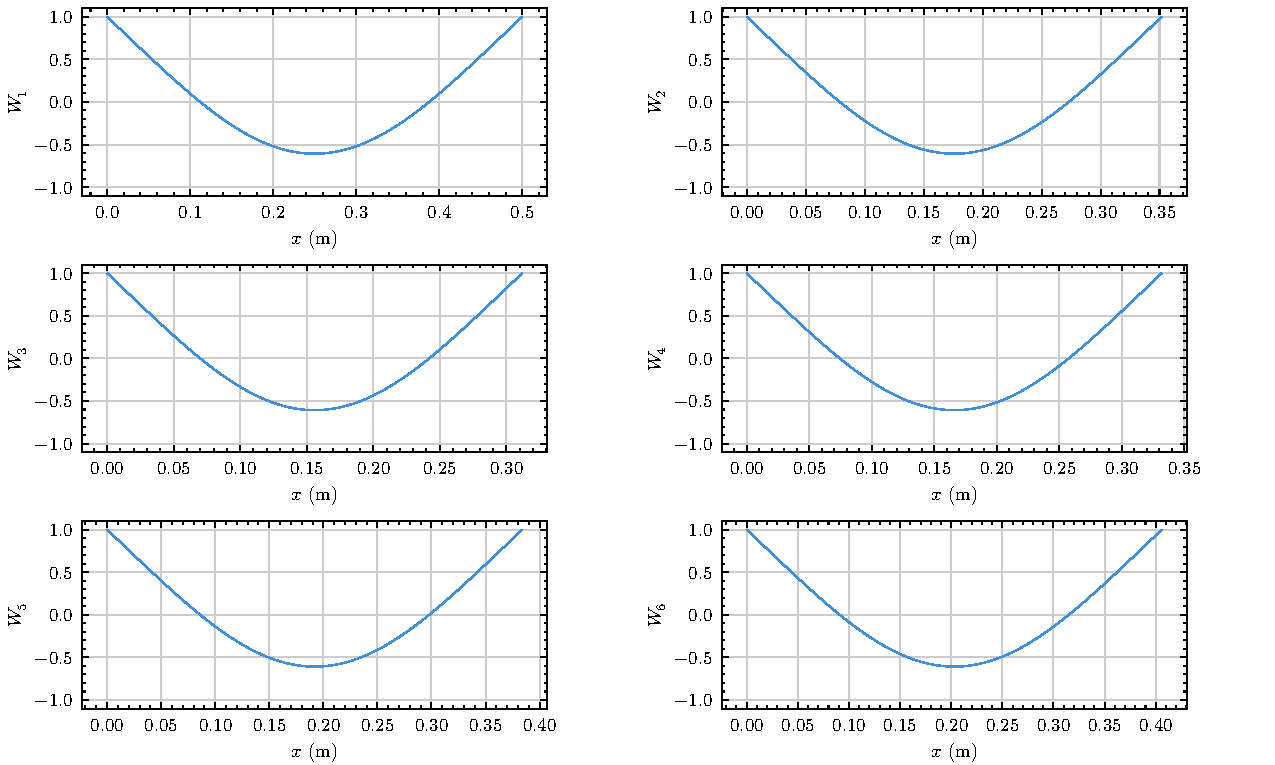
\includegraphics[width=0.95\linewidth]{figures/generated/solutions/C2.pdf}
\caption{First flexible mode for each tube, normalized by maximum absolute displacement.}
\end{figure}
The mode shape is the same function of \(x/L\) for all six tubes, but each plot uses its measured physical length.

For graduate tuning, select the nearest natural note without a sharp. Since frequency decreases as length increases, trial lengths are increased for tubes 1, 2, 4, 5, and 6, and decreased for tube 3. The relation $f_1\propto L^{-2}$ follows because the tubes share the same material and cross section. For example, tube 1 at 505 mm gives 525.343 Hz and at 506 mm gives 523.269 Hz, approaching the C5 target of 523.251 Hz as length increases. The table shows two manual trials and the refined length from \(L_*=\sqrt{a^2z_1^2/(2\pi f_{\rm target})}\).
\begin{center}\small\begin{tabular}{lrrrrrr}\toprule
Tube & Target & Target (Hz) & Trial 1 (mm, Hz) & Trial 2 (mm, Hz) & \(L_*\) (mm)\\\midrule
1&C5&523.251&505, 525.343&506, 523.269&506.0085\\
2&C6&1046.502&357, 1051.210&358, 1045.345&357.8020\\
3&F6&1396.913&310, 1394.127&309.7, 1396.829&309.6907\\
4&D6&1174.659&337, 1179.685&338, 1172.715&337.7201\\
5&A5&880.000&390, 880.839&390.2, 879.936&390.1859\\
6&G5&783.991&413, 785.463&413.4, 783.944&413.3875\\\bottomrule\end{tabular}\end{center}
These values use the free--free model and the specified material and geometry. The MATLAB script calculates the roots, note frequencies, node comparisons, and mode shapes.
\lstinputlisting[style=hwmatlab]{matlab/C2.m}
